\documentclass{beamer}
\usetheme{Madrid}
\usecolortheme{beaver}

\usepackage[utf8]{inputenc}
\usepackage{amsmath}
\usepackage{tikz}
\usetikzlibrary{arrows.meta, positioning}

\tikzset{
    bnode/.style={circle, draw, thick, fill=black, text=white, minimum size=7mm, font=\footnotesize\bfseries},
    rnode/.style={circle, draw, thick, fill=red!80!black, text=white, minimum size=7mm, font=\footnotesize\bfseries},
    nilnode/.style={rectangle, draw, fill=black, text=white, minimum size=3mm, font=\tiny},
    edge from parent/.style={draw, thick, -Latex},
}

\title{Red-Black Trees: Insertion and Rebalancing}
\subtitle{BLG 202E -- Data Structures}
\author{Deniz Sipahi -- 150230006}
\date{May 11, 2026}
\institute{Istanbul Technical University}

\begin{document}

% ============================================================
% Slide 1 -- Title
% ============================================================
\begin{frame}
\titlepage
\end{frame}

% ============================================================
% Slide 2 -- Motivation
% ============================================================
\begin{frame}{1. Motivation -- Why Balance Matters}
\begin{itemize}
    \item A \textbf{Binary Search Tree (BST)} supports search, insert, and delete in $O(h)$ time, where $h$ is the tree height.
    \item In the \textbf{worst case}, a BST degenerates into a linked list:
    \begin{itemize}
        \item $h = n \Rightarrow$ operations become $O(n)$.
    \end{itemize}
    \item A \textbf{balanced BST} guarantees $h = O(\log n)$, making all operations efficient.
    \item \textbf{Red-Black Trees} are one of the most widely used self-balancing BSTs --- used in the Linux kernel, Java's \texttt{TreeMap}, and C++ \texttt{std::map}.
\end{itemize}

\begin{block}{Key Insight}
Balancing is not free --- it requires extra bookkeeping. Red-Black Trees achieve this through \textbf{coloring constraints} and \textbf{rotations}, guaranteeing $O(\log n)$ worst-case height.
\end{block}
\end{frame}

% ============================================================
% Slide 3 -- Red-Black Tree Properties
% ============================================================
\begin{frame}{2. Red-Black Tree Properties}
Every Red-Black Tree satisfies these five invariants:
\begin{enumerate}
    \item Every node is either \textcolor{red}{\textbf{RED}} or \textbf{BLACK}.\\
          {\small\textit{This binary labeling gives us a simple mechanism to enforce balance.}}
    \item The root is always \textbf{BLACK}.\\
          {\small\textit{This anchors the tree --- no violation can ``escape'' past the root.}}
    \item Every leaf (NIL/null) is \textbf{BLACK}.\\
          {\small\textit{Treating NILs as black simplifies the counting in Property 5.}}
    \item If a node is \textcolor{red}{\textbf{RED}}, both its children must be \textbf{BLACK}.\\
          {\small\textit{This prevents long chains of RED nodes, bounding the longest path.}}
    \item All paths from a node to its descendant leaves have the same \textbf{black-height}.\\
          {\small\textit{This is the core balance invariant --- it guarantees $O(\log n)$ height.}}
\end{enumerate}
\end{frame}

% ============================================================
% Slide 4 -- Node Structure (TikZ box diagram)
% ============================================================
\begin{frame}{3. Node Structure}
Each node in a Red-Black Tree stores five components:

\vspace{0.5em}
\begin{center}
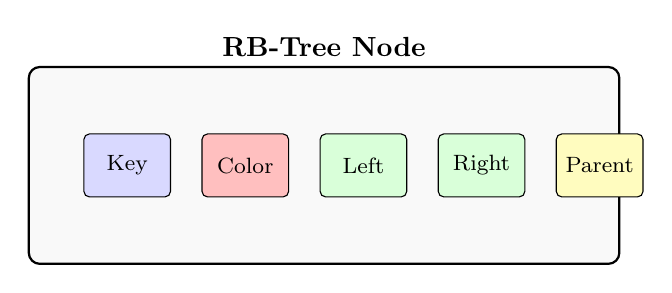
\begin{tikzpicture}
    \node[draw, rounded corners, minimum width=7.5cm, minimum height=2.5cm, fill=gray!5, thick] (box) {};
    \node[above] at (box.north) {\textbf{RB-Tree Node}};
    \node[draw, fill=blue!15, minimum width=1.1cm, minimum height=0.8cm, rounded corners=2pt] (k) at (-2.5,0) {\footnotesize Key};
    \node[draw, fill=red!25, minimum width=1.1cm, minimum height=0.8cm, rounded corners=2pt] (c) at (-1.0,0) {\footnotesize Color};
    \node[draw, fill=green!15, minimum width=1.1cm, minimum height=0.8cm, rounded corners=2pt] (l) at (0.5,0) {\footnotesize Left};
    \node[draw, fill=green!15, minimum width=1.1cm, minimum height=0.8cm, rounded corners=2pt] (r) at (2.0,0) {\footnotesize Right};
    \node[draw, fill=yellow!25, minimum width=1.1cm, minimum height=0.8cm, rounded corners=2pt] (p) at (3.5,0) {\footnotesize Parent};
\end{tikzpicture}
\end{center}

\vspace{0.3em}
\begin{itemize}
    \item \textbf{Key}: the stored value used for BST ordering
    \item \textbf{Color}: RED or BLACK --- used to maintain balance invariants
    \item \textbf{Left / Right}: pointers to child subtrees
    \item \textbf{Parent}: pointer to the parent (needed for fix-up traversal upward)
\end{itemize}
\end{frame}

% ============================================================
% Slide 5 -- Insertion Base Steps
% ============================================================
\begin{frame}{4. Insertion -- Base Steps}
Inserting into a Red-Black Tree follows two phases:

\begin{enumerate}
    \item \textbf{Standard BST Insert}: Insert the new node as a leaf, colored \textcolor{red}{\textbf{RED}}.
    \item \textbf{Fix-up Phase}: Restore any violated RB-tree properties.
\end{enumerate}

\vspace{0.5em}
\pause
Possible violations after inserting a RED node:
\begin{itemize}
    \item \textbf{Property 2 violation}: The new node might be the root (root must be BLACK).\\
          {\small Fix: simply recolor the root to BLACK.}
    \item \textbf{Property 4 violation}: The new node's parent might also be RED.\\
          {\small Fix: apply one of the three fix-up cases (next slides).}
\end{itemize}

\begin{block}{Why insert as RED?}
Inserting as RED preserves Property 5 (black-height) automatically. We only risk violating Property 4, which is easier to fix locally.
\end{block}
\end{frame}

% ============================================================
% Slide 6 -- Fix-up Cases 1 & 2 (TikZ diagram)
% ============================================================
\begin{frame}{5. Fix-up Cases 1 \& 2}
\textbf{Case 1 --- Uncle is RED (Recoloring):}
\begin{itemize}
    \item Recolor parent and uncle to BLACK, grandparent to RED.
    \item \textit{Intuition: push the ``redness problem'' up the tree --- adding redness at a higher level creates fewer local violations.}
    \item Move the pointer up to grandparent and repeat fix-up.
\end{itemize}

\vspace{0.2em}
\pause
\textbf{Case 2 --- Uncle is BLACK, zig-zag (Rotation):}
\begin{itemize}
    \item The new node is on the \emph{opposite side} of its parent relative to grandparent.
    \item Perform a rotation on the parent to straighten the path $\rightarrow$ converts to Case 3.
\end{itemize}

\vspace{0.2em}
\begin{center}
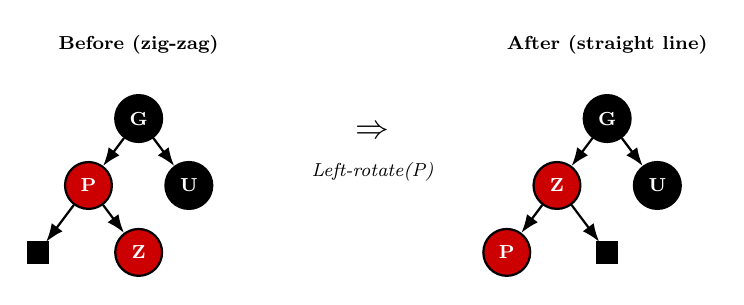
\begin{tikzpicture}[level distance=10mm, sibling distance=15mm, scale=0.85, transform shape]
    % Before rotation
    \node at (-2.5, 1.6) {\footnotesize \textbf{Before (zig-zag)}};
    \node[bnode] (g1) at (-2.5, 0.5) {G}
        child { node[rnode] (p1) {P}
            child { node[nilnode] {} }
            child { node[rnode] (z1) {Z} }
        }
        child { node[bnode] (u1) {U} };

    % Arrow
    \node at (1.0, 0.3) {\Large $\Rightarrow$};
    \node at (1.0, -0.3) {\footnotesize \textit{Left-rotate(P)}};

    % After rotation
    \node at (4.5, 1.6) {\footnotesize \textbf{After (straight line)}};
    \node[bnode] (g2) at (4.5, 0.5) {G}
        child { node[rnode] (z2) {Z}
            child { node[rnode] (p2) {P} }
            child { node[nilnode] {} }
        }
        child { node[bnode] (u2) {U} };
\end{tikzpicture}
\end{center}

\footnotesize{Note: the symmetric (right-subtree) case is a mirror image of the above.}
\end{frame}

% ============================================================
% Slide 7 -- Fix-up Case 3 + Worked Example with \pause
% The example: insert 15 into {7B, 3R, 18R, 10B, 22B, 26B, 8R, 11R}
% This triggers Case 1 (uncle 22 is RED) -> recolor -> propagates up
% ============================================================
\begin{frame}{6. Fix-up Case 3 + Worked Example}
\textbf{Case 3 --- Uncle is BLACK, straight line (Rotate + Recolor):}
\begin{itemize}
    \item Rotate on the grandparent in the opposite direction.
    \item Swap colors of parent and grandparent.
\end{itemize}

\vspace{0.3em}
\textbf{Example:} Insert value \textbf{15} into tree $\{10_B,\ 5_R,\ 20_R,\ 3_B,\ 7_B,\ 17_B,\ 25_B\}$:

\begin{center}
\only<1>{%
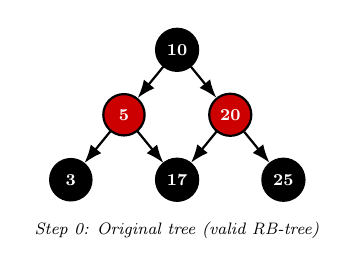
\begin{tikzpicture}[level distance=11mm, sibling distance=18mm, scale=0.75, transform shape]
    \node[bnode] {10}
        child { node[rnode] {5}
            child { node[bnode] {3} }
            child { node[bnode] {7} }
        }
        child { node[rnode] {20}
            child { node[bnode] {17} }
            child { node[bnode] {25} }
        };
    \node[below, font=\footnotesize] at (0,-2.8) {\textit{Step 0: Original tree (valid RB-tree)}};
\end{tikzpicture}
}%
\only<2>{%
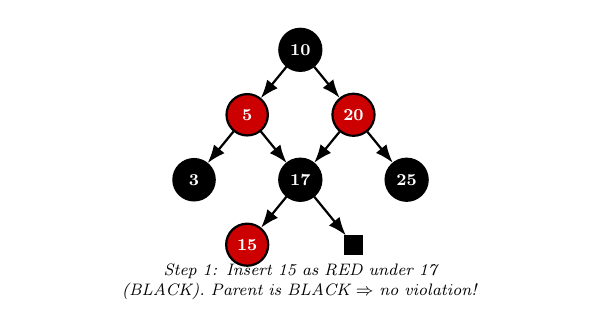
\begin{tikzpicture}[level distance=11mm, sibling distance=18mm, scale=0.75, transform shape]
    \node[bnode] {10}
        child { node[rnode] {5}
            child { node[bnode] {3} }
            child { node[bnode] {7} }
        }
        child { node[rnode] {20}
            child { node[bnode] {17}
                child { node[rnode] {15} }
                child { node[nilnode] {} }
            }
            child { node[bnode] {25} }
        };
    \node[below, font=\footnotesize, text width=9cm, align=center] at (0,-3.5) {\textit{Step 1: Insert 15 as RED under 17 (BLACK). Parent is BLACK $\Rightarrow$ no violation!}};
\end{tikzpicture}
}%
\only<3>{%
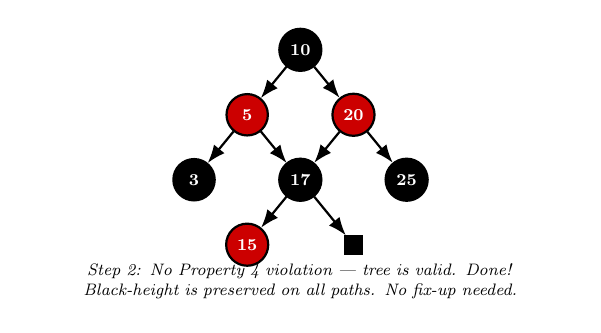
\begin{tikzpicture}[level distance=11mm, sibling distance=18mm, scale=0.75, transform shape]
    \node[bnode] {10}
        child { node[rnode] {5}
            child { node[bnode] {3} }
            child { node[bnode] {7} }
        }
        child { node[rnode] {20}
            child { node[bnode] {17}
                child { node[rnode] {15} }
                child { node[nilnode] {} }
            }
            child { node[bnode] {25} }
        };
    \node[below, font=\footnotesize, text width=9cm, align=center] at (0,-3.5) {\textit{Step 2: No Property 4 violation --- tree is valid. Done!}\\
    \textit{Black-height is preserved on all paths. No fix-up needed.}};
\end{tikzpicture}
}%
\end{center}
\end{frame}

% ============================================================
% Slide 8 -- Summary & Key Takeaways
% ============================================================
\begin{frame}{7. Summary \& Key Takeaways}
Red-Black Trees maintain balance through \textbf{3 fix-up cases} after insertion:

\begin{enumerate}
    \item \textbf{Recolor} --- uncle is RED $\rightarrow$ push the problem upward.\\
          {\small Mnemonic: \textit{``Uncle RED? Recolor and ascend.''}}
    \item \textbf{Rotate to straighten} --- zig-zag path, uncle is BLACK $\rightarrow$ convert to Case 3.\\
          {\small Mnemonic: \textit{``Zig-zag? Rotate to align.''}}
    \item \textbf{Rotate + recolor} --- straight line, uncle is BLACK $\rightarrow$ final fix.\\
          {\small Mnemonic: \textit{``Straight line? Rotate the grandparent, done.''}}
\end{enumerate}

\vspace{0.5em}
\begin{block}{Complexity}
Insert, delete, and search all run in $\mathbf{O(\log n)}$ time. Fix-up requires at most \textbf{2 rotations} and $O(\log n)$ recolorings.
\end{block}

\vspace{0.3em}
\begin{block}{Real-World Analogy}
Think of a Red-Black Tree as a corporate hierarchy: RED employees must always report to BLACK managers. When two RED employees end up adjacent, we either promote someone (recolor) or reorganize the team (rotate) until the reporting structure is restored.
\end{block}

\footnotesize{Reference: Cormen et al., \textit{Introduction to Algorithms}, 4th Ed., Chapter 13.}
\end{frame}

\end{document}
